\section{SAME - Sistema de Aquisição do Motor Elétrico}
\label{sec:same}

O Sistema de Aquisição do Motor Elétrico (SAME) mede as tensões e correntes de
fase do motor e executa embarcado o Observador por Modos Deslizantes (SMO).

A cadeia de medição foi dividida em dois caminhos independentes --- corrente e
tensão de fase ---, cada um projetado para entregar ao conversor
analógico-digital (ADC) do CH32V307 um sinal na faixa de entrada do periférico,
preservando a coerência de fase entre os dois caminhos exigida pelo observador
(\autoref{sec:same_condicionamento}). Os dois caminhos ficam numa placa de
condicionamento própria, a AQ1, por onde passam as três fases do motor; o
roteamento dela está na \autoref{fig:pcb_same}. As seis saídas da AQ1 chegam
à placa de desenvolvimento do microcontrolador, montada sobre placa
perfurada como na SIBA, com a pinagem da \autoref{fig:pinagem_same}: o
primeiro conversor lê as três correntes e o segundo as três tensões,
pareados por fase, de modo que a corrente e a tensão de uma mesma fase são
amostradas no mesmo instante.

\begin{figure}[H]
    \centering
    \caption{Roteamento da placa de condicionamento AQ1 da SAME}
    \label{fig:pcb_same}
    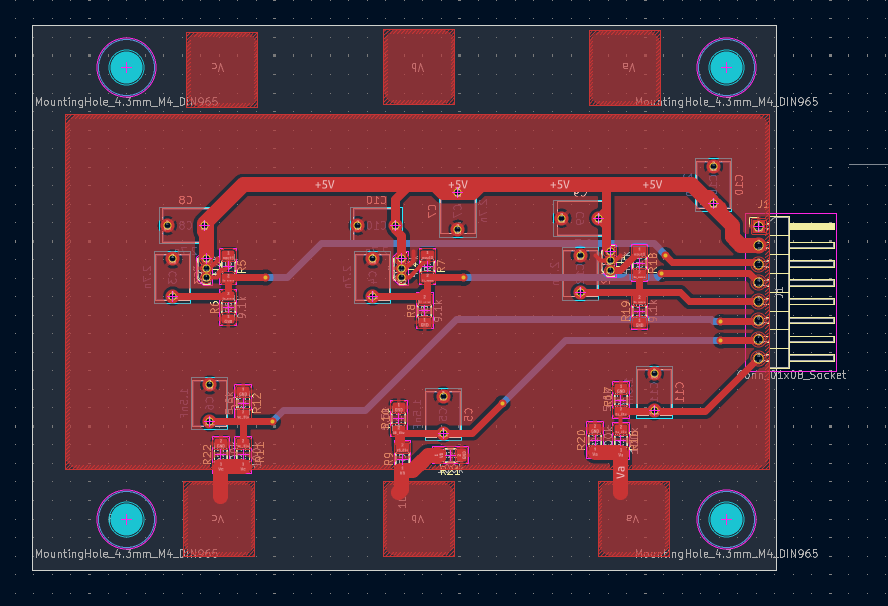
\includegraphics[width=0.85\textwidth]{Textuais/Imgs/Metodologia/placa aq1 SAME.png}

    Fonte: Autor (2026)
\end{figure}

\begin{figure}[H]
    \centering
    \caption{Pinagem da SAME na placa de desenvolvimento do CH32V307VCT6}
    \label{fig:pinagem_same}
    \resizebox{\textwidth}{!}{% Gerado a partir de "Imgs/Montagem croqui.xlsx" (aba micro) + pinagem do firmware.
\begin{tikzpicture}[font=\fontsize{7}{8}\selectfont, every node/.append style={font=\fontsize{7}{8}\selectfont},
  pin/.style={draw, minimum width=0.56cm, minimum height=0.36cm, inner sep=0pt, font=\fontsize{4.6}{5}\selectfont\sffamily},
  p-pwr/.style={pin, fill=gray!35}, p-free/.style={pin, fill=white, text=gray},
  p-adc/.style={pin, fill=orange!45}, p-nm/.style={pin, fill=orange!15, dashed, text=gray},
  p-dig/.style={pin, fill=cyan!30}, p-com/.style={pin, fill=green!30}, p-seg/.style={pin, fill=red!35}, p-res/.style={pin, fill=white, dashed},
  d/.style={inner sep=1pt}, d-nm/.style={d, text=gray, font=\fontsize{7}{8}\selectfont\itshape}, d-res/.style={d, text=gray}]
  \draw[rounded corners=3pt, very thick, fill=black!4] (-0.38,0.5) rectangle (9.0,-10.16);
  \node[font=\fontsize{9}{10}\selectfont\bfseries] at (4.31,0.85) {SAME};
  \node[draw, fill=white, minimum width=2.2cm, minimum height=0.7cm, font=\fontsize{5}{6}\selectfont] at (4.31,-9.5) {conector Ethernet};
  \node[draw, fill=white, minimum width=1.7cm, minimum height=1.1cm, font=\fontsize{5}{6}\selectfont, align=center] at (4.6,-2.4) {CH32V307VCT6};
  \node[p-pwr] at (0.00,0.00) {GND};
  \node[p-pwr] at (0.62,0.00) {GND};
  \node[p-pwr] at (0.00,-0.42) {GND};
  \node[p-pwr] at (0.62,-0.42) {GND};
  \node[p-free] at (0.00,-0.84) {PE0};
  \node[p-free] at (0.62,-0.84) {PE1};
  \node[p-free] at (0.00,-1.26) {PE2};
  \node[p-free] at (0.62,-1.26) {PE3};
  \node[p-free] at (0.00,-1.68) {PE4};
  \node[p-free] at (0.62,-1.68) {PE5};
  \node[p-free] at (0.00,-2.10) {PE6};
  \node[p-free] at (0.62,-2.10) {PC13};
  \node[p-free] at (0.00,-2.52) {PC14};
  \node[p-free] at (0.62,-2.52) {PC15};
  \node[p-adc] at (0.00,-2.94) {PC0};
  \node[d, anchor=east] at (-0.50,-2.94) {Tensão fase $c$ (ADC2)};
  \node[p-adc] at (0.62,-2.94) {PC1};
  \node[d, anchor=west] at (0.96,-2.94) {Tensão fase $b$ (ADC2)};
  \node[p-adc] at (0.00,-3.36) {PC2};
  \node[d, anchor=east] at (-0.50,-3.36) {Tensão fase $a$ (ADC2)};
  \node[p-free] at (0.62,-3.36) {PC3};
  \node[p-adc] at (0.00,-3.78) {PA0};
  \node[d, anchor=east] at (-0.50,-3.78) {Corrente fase $c$ (ADC1)};
  \node[p-adc] at (0.62,-3.78) {PA1};
  \node[d, anchor=west] at (0.96,-3.78) {Corrente fase $b$ (ADC1)};
  \node[p-free] at (0.00,-4.20) {PA2};
  \node[p-adc] at (0.62,-4.20) {PA3};
  \node[d, anchor=west] at (0.96,-4.20) {Corrente fase $a$ (ADC1)};
  \node[p-free] at (0.00,-4.62) {PA4};
  \node[p-free] at (0.62,-4.62) {PA5};
  \node[p-free] at (0.00,-5.04) {PA6};
  \node[p-free] at (0.62,-5.04) {PA7};
  \node[p-free] at (0.00,-5.46) {PC4};
  \node[p-free] at (0.62,-5.46) {PC5};
  \node[p-free] at (0.00,-5.88) {PB0};
  \node[p-free] at (0.62,-5.88) {PB1};
  \node[p-free] at (0.00,-6.30) {PB2};
  \node[p-free] at (0.62,-6.30) {PE7};
  \node[p-free] at (0.00,-6.72) {PE8};
  \node[p-free] at (0.62,-6.72) {PE9};
  \node[p-free] at (0.00,-7.14) {PE10};
  \node[p-free] at (0.62,-7.14) {PE11};
  \node[p-free] at (0.00,-7.56) {PE12};
  \node[p-free] at (0.62,-7.56) {PE13};
  \node[p-free] at (0.00,-7.98) {PE14};
  \node[p-free] at (0.62,-7.98) {PE15};
  \node[p-com] at (0.00,-8.40) {PB10};
  \node[d, anchor=east] at (-0.50,-8.40) {I2C2 SCL (EEPROM)};
  \node[p-com] at (0.62,-8.40) {PB11};
  \node[d, anchor=west] at (0.96,-8.40) {I2C2 SDA (EEPROM)};
  \node[p-pwr] at (0.00,-8.82) {GND};
  \node[p-pwr] at (0.62,-8.82) {3V3};
  \node[p-pwr] at (0.00,-9.24) {GND};
  \node[p-pwr] at (0.62,-9.24) {3V3};
  \node[p-pwr] at (0.00,-9.66) {GND};
  \node[p-pwr] at (0.62,-9.66) {3V3};
  \node[p-pwr] at (8.00,0.00) {3V3};
  \node[p-pwr] at (8.62,0.00) {GND};
  \node[p-pwr] at (8.00,-0.42) {VBAT};
  \node[p-pwr] at (8.62,-0.42) {GND};
  \node[p-free] at (8.00,-0.84) {PB9};
  \node[p-free] at (8.62,-0.84) {PB8};
  \node[p-free] at (8.00,-1.26) {PB7};
  \node[p-free] at (8.62,-1.26) {PB6};
  \node[p-free] at (8.00,-1.68) {PB5};
  \node[p-dig] at (8.62,-1.68) {PB4};
  \node[d, anchor=west] at (8.96,-1.68) {LED verde};
  \node[p-free] at (8.00,-2.10) {PB3};
  \node[p-free] at (8.62,-2.10) {PD7};
  \node[p-free] at (8.00,-2.52) {PD6};
  \node[p-free] at (8.62,-2.52) {PD5};
  \node[p-free] at (8.00,-2.94) {PD4};
  \node[p-free] at (8.62,-2.94) {PD3};
  \node[p-free] at (8.00,-3.36) {PD2};
  \node[p-free] at (8.62,-3.36) {PD1};
  \node[p-free] at (8.00,-3.78) {PD0};
  \node[p-free] at (8.62,-3.78) {PC12};
  \node[p-free] at (8.00,-4.20) {PC11};
  \node[p-free] at (8.62,-4.20) {PC10};
  \node[p-dig] at (8.00,-4.62) {PA15};
  \node[d, anchor=east] at (7.66,-4.62) {LED vermelho};
  \node[p-free] at (8.62,-4.62) {PA14};
  \node[p-free] at (8.00,-5.04) {PA13};
  \node[p-free] at (8.62,-5.04) {PA12};
  \node[p-free] at (8.00,-5.46) {PA11};
  \node[p-com] at (8.62,-5.46) {PA10};
  \node[d, anchor=west] at (8.96,-5.46) {USART1 RX};
  \node[p-com] at (8.00,-5.88) {PA9};
  \node[d, anchor=east] at (7.66,-5.88) {USART1 TX};
  \node[p-free] at (8.62,-5.88) {PA8};
  \node[p-com] at (8.00,-6.30) {PC9};
  \node[d, anchor=east] at (7.66,-6.30) {Ethernet TX$-$};
  \node[p-com] at (8.62,-6.30) {PC8};
  \node[d, anchor=west] at (8.96,-6.30) {Ethernet TX+};
  \node[p-com] at (8.00,-6.72) {PC7};
  \node[d, anchor=east] at (7.66,-6.72) {Ethernet RX$-$};
  \node[p-com] at (8.62,-6.72) {PC6};
  \node[d, anchor=west] at (8.96,-6.72) {Ethernet RX+};
  \node[p-free] at (8.00,-7.14) {PD15};
  \node[p-free] at (8.62,-7.14) {PD14};
  \node[p-free] at (8.00,-7.56) {PD13};
  \node[p-free] at (8.62,-7.56) {PD12};
  \node[p-free] at (8.00,-7.98) {PD11};
  \node[p-free] at (8.62,-7.98) {PD10};
  \node[p-free] at (8.00,-8.40) {PD9};
  \node[p-free] at (8.62,-8.40) {PD8};
  \node[p-free] at (8.00,-8.82) {PB15};
  \node[p-free] at (8.62,-8.82) {PB14};
  \node[p-free] at (8.00,-9.24) {PB13};
  \node[p-free] at (8.62,-9.24) {PB12};
  \node[p-pwr] at (8.00,-9.66) {5V};
  \node[p-pwr] at (8.62,-9.66) {GND};
  % legenda (centralizada sob a placa)
  \begin{scope}[local bounding box=leg, shift={(0,-10.75)}]
    \node[p-adc, minimum width=0.4cm] (l0) at (0,0) {};
    \node[d, right=2pt of l0] (t0) {Analógico (ADC)};
    \node[p-dig, minimum width=0.4cm, right=10pt of t0] (l1)  {};
    \node[d, right=2pt of l1] (t1) {E/S digital};
    \node[p-com, minimum width=0.4cm, right=10pt of t1] (l2)  {};
    \node[d, right=2pt of l2] (t2) {Comunicação};
    \node[p-pwr, minimum width=0.4cm, right=10pt of t2] (l3)  {};
    \node[d, right=2pt of l3] (t3) {Alimentação};
  \end{scope}
\end{tikzpicture}
}

    Fonte: Autor (2026)
\end{figure}

\subsection{Medição de Tensão e Corrente de Fase}
\label{sec:same_tensao}
\label{sec:same_condicionamento}

A aquisição usa os dois conversores do CH32V307 em modo dual simultâneo: o
primeiro converte as três correntes de fase e o segundo, as três tensões,
disparados pelo mesmo evento. A corrente e a tensão de uma mesma fase são
amostradas no mesmo instante, condição para a transformada de Clarke e para o
observador, que as confrontam amostra a amostra.

A taxa de amostragem parte do critério de Nyquist: para que um sinal de banda
limitada a $f_{max}$ possa ser reconstruído sem rebatimento, a amostragem deve
ocorrer a $f_s > 2 f_{max}$ \cite{oppenheim2009}. O conteúdo que interessa ao
observador é a fundamental elétrica e as raias de chaveamento do ESC, em
\SI{8}{\kilo\hertz}; portanto, a taxa de quadro precisa ficar bem acima de
\SI{16}{\kilo\hertz}.

A \autoref{fig:adc_clock_quadro} mostra como essa taxa é obtida. O
\textit{clock} do conversor é limitado a \SI{14}{\mega\hertz}
(\autoref{tab:adc_specs}) e deriva do barramento de periféricos por um
divisor que admite apenas as razões \num{2}, \num{4}, \num{6} e \num{8}. Com o
barramento a \SI{144}{\mega\hertz}, o menor valor possível seria
\SI{18}{\mega\hertz}, acima do limite; reduzindo o barramento à metade
(\SI{72}{\mega\hertz}) e dividindo por \num{6}, o conversor opera a
\SI{12}{\mega\hertz}. Cada canal gasta \num{28,5} ciclos de amostragem e
\num{11} de conversão, e o quadro com as três fases soma \num{118,5} ciclos,
ou \SI{9,875}{\micro\second}. A taxa de quadro é de \SI{101}{\kilo\hertz}
(banda útil de \SI{50}{\kilo\hertz}), e é ela que define o período $T_s$ do
observador.

\begin{figure}[H]
    \centering
    \caption{Cadeia de \textit{clock} do conversor e temporização de um quadro de aquisição}
    \label{fig:adc_clock_quadro}
    \begin{tikzpicture}[font=\small, >=Stealth,
        blk/.style={draw, rounded corners=2pt, align=center, minimum height=0.9cm, inner sep=3pt},
        amo/.style={draw, fill=cyan!25, minimum height=0.55cm, inner sep=0pt},
        conv/.style={draw, fill=orange!35, minimum height=0.55cm, inner sep=0pt}]
        % cadeia de clock
        \node[blk] (sys) at (0,0) {Sistema\\\SI{144}{\mega\hertz}};
        \node[blk] (apb) at (3.6,0) {Barramento de\\periféricos \SI{72}{\mega\hertz}};
        \node[blk] (adc) at (7.6,0) {\textit{Clock} do ADC\\\SI{12}{\mega\hertz}};
        \node[blk] (con) at (11.2,0) {ADC1 + ADC2\\(dual)};
        \draw[->, thick] (sys) -- node[above, font=\scriptsize] {$\div 2$} (apb);
        \draw[->, thick] (apb) -- node[above, font=\scriptsize] {$\div 6$} (adc);
        \draw[->, thick] (adc) -- (con);
        % temporização do quadro (39,5 ciclos por fase -> 3,6 cm)
        \def\ua{2.597}\def\ub{1.003}
        \foreach \k/\i/\v in {0/a/a,1/b/b,2/c/c} {
            \pgfmathsetmacro{\xo}{\k*3.6}
            \node[amo, minimum width=\ua cm, anchor=west] at (\xo,-2.0) {$i_\i$};
            \node[conv, minimum width=\ub cm, anchor=west] at (\xo+\ua,-2.0) {};
            \node[amo, minimum width=\ua cm, anchor=west] at (\xo,-2.75) {$v_\v$};
            \node[conv, minimum width=\ub cm, anchor=west] at (\xo+\ua,-2.75) {};
        }
        \node[anchor=east, font=\scriptsize] at (-0.1,-2.0) {ADC1};
        \node[anchor=east, font=\scriptsize] at (-0.1,-2.75) {ADC2};
        \draw[decorate, decoration={brace, mirror, amplitude=5pt}] (0,-3.15) -- (10.8,-3.15)
            node[midway, below=6pt, font=\scriptsize] {quadro: \num{118,5} ciclos $=\SI{9,875}{\micro\second}=T_s$ \quad ($f_s\approx\SI{101}{\kilo\hertz}$)};
        \draw[decorate, decoration={brace, amplitude=4pt}] (0,-1.6) -- (\ua,-1.6)
            node[midway, above=4pt, font=\scriptsize] {amostragem: \num{28,5} ciclos};
        \draw[decorate, decoration={brace, amplitude=4pt}] (\ua,-1.6) -- (3.6,-1.6)
            node[midway, above=14pt, font=\scriptsize] {conversão: \num{11}};
    \end{tikzpicture}

    Fonte: Autor (2026)
\end{figure}

\begin{table}[h]
\centering
\caption{Características do ADC 12-bit do CH32V307.}
\label{tab:adc_specs}
\begin{tabular}{lccccc}
\hline
\textbf{Parâmetro} & \textbf{Símbolo} & \textbf{Min.} & \textbf{Typ.} & \textbf{Máx.} & \textbf{Unidade} \\
\hline
Frequência de clock ADC & $f_{ADC}$ & -- & -- & 14 & MHz \\
Taxa de amostragem & $f_S$ & 0,05 & -- & 1 & MHz \\
Faixa de conversão & $V_{AIN}$ & 0 & -- & $V_{REF+}$ & V \\
Impedância de entrada externa & $R_{AIN}$ & -- & -- & 50 & k$\Omega$ \\
Tempo de amostragem & $t_s$ & 1,5 & -- & 239,5 & $1/f_{ADC}$ \\
Tempo total de conversão & $t_{CONV}$ & 14 & -- & 252 & $1/f_{ADC}$ \\
Erro de \textit{offset} & $E_O$ & -- & -- & ±2 & LSB \\
Não-linearidade integral & $E_L$ & -- & -- & ±4 & LSB \\
\hline
\multicolumn{6}{l}{\small \textit{Fonte: WCH CH32V307 Datasheet \cite{ch32v307_datasheet}}} \\
\end{tabular}
\end{table}

Os \num{28,5} ciclos de amostragem são o maior valor tabelado que mantém o
quadro em \SI{10}{\micro\second}. Esse tempo também limita a impedância da
fonte ligada ao conversor, para que o erro de amostragem fique abaixo de
$1/4$ LSB \cite{ch32v307_datasheet}:

\begin{equation}
R_{AIN} < \frac{t_s}{f_{ADC} \cdot C_{ADC} \cdot \ln(2^{N+2})} - R_{ADC},
\label{eq:rain_max}
\end{equation}

\noindent com $N = 12$~bits, $C_{ADC} = \SI{8}{\pico\farad}$ e
$R_{ADC} \approx \SI{0,8}{\kilo\ohm}$, o que dá
$R_{AIN} < \SI{25,2}{\kilo\ohm}$ para \num{28,5} ciclos. O erro de
\textit{offset} é removido na calibração; a não-linearidade, de até
±4~LSB, é limitação do próprio conversor.

\subsubsection{Medição de Tensão de Fase}
\label{sec:same_divisor_tensao}

Cada tensão de fase é medida em relação ao terra do sistema, que é o mesmo
terminal negativo do barramento de potência, e chega ao ADC por um divisor
resistivo com capacitor (\autoref{fig:cond_tensao}), que estabelece também o
filtro \textit{antialiasing} da aquisição.

\begin{figure}[H]
    \centering
    \caption{Condicionamento do caminho de tensão de fase}
    \label{fig:cond_tensao}
    \begin{circuitikz}[american, scale=1.0, transform shape]
        \draw (0,0) node[left] {$V_{fase}$} to[short, o-] (0.8,0);
        \draw (0.8,0) to[R, l=$R_1$, a=\SI{130}{\kilo\ohm}] (3.6,0);
        \draw (3.6,0) to[R, l_=$R_2$, a^=\SI{7,5}{\kilo\ohm}] (3.6,-2.4);
        \draw (3.6,-2.4) node[ground]{};
        \draw (3.6,0) -- (5.6,0);
        \draw (5.6,0) to[C, l_=$C$] (5.6,-2.4);
        \draw (5.6,-2.4) -- (3.6,-2.4);
        \draw (5.6,0) to[short, -o] (7.0,0) node[right] {$V_{ADC}$};
    \end{circuitikz}

    Fonte: Autor (2026)
\end{figure}

A atenuação do divisor é dada pela \autoref{eq:cond_k} e a frequência de corte
do filtro pela \autoref{eq:cond_fc}.

\begin{equation}
k = \frac{R_2}{R_1 + R_2}
\label{eq:cond_k}
\end{equation}

\begin{equation}
f_c = \frac{1}{2\pi \left(R_1 \parallel R_2\right) C}
    = \frac{R_1 + R_2}{2\pi\,R_1 R_2\,C}
\label{eq:cond_fc}
\end{equation}

\noindent
Com $R_1 = \SI{130}{\kilo\ohm}$ e $R_2 = \SI{7,5}{\kilo\ohm}$ resulta
$k = 0{,}0545$, o que coloca o fundo de escala da medição em \SI{60,5}{\volt} ---
pouco mais do dobro da tensão de barramento, folga adotada para o sobressinal de
comutação --- e a resolução em \SI{14,8}{\milli\volt} por LSB.

A resistência equivalente do divisor é de \SI{7,09}{\kilo\ohm}, abaixo do limite
de \SI{25,2}{\kilo\ohm} que a \autoref{eq:rain_max} impõe ao tempo de
amostragem adotado, de \num{28,5} ciclos.

Fixadas as resistências, o capacitor é o único grau de liberdade que resta, e
seu valor decorre da frequência de corte adotada.

O divisor consome \SI{218}{\micro\ampere} com o
barramento em \SI{30}{\volt}, dissipando \SI{6,2}{\milli\watt} em $R_1$.

Como não há amplificador isolando o divisor do conversor, a corrente que
recarrega o capacitor de amostragem do ADC atravessa a resistência equivalente
do divisor. O efeito é o erro de ganho da \autoref{eq:cond_ganho}. Por ser
proporcional ao sinal, é absorvido na calibração.

\begin{equation}
\varepsilon_{ganho} = \left(R_1 \parallel R_2\right) f_S\,C_{ADC}
= \SI{7,09}{\kilo\ohm} \times \SI{101}{\kilo\hertz} \times \SI{8}{\pico\farad}
= \SI{0,57}{\percent}
\label{eq:cond_ganho}
\end{equation}


\subsubsection{Sensor de Corrente com Núcleo Toroidal}
\label{sec:same_sensor_corrente}

O sensor Hall utilizado é o SS49E, linear e ratiométrico
\cite{ramsden2006}: a tensão de saída varia linearmente com a densidade de
fluxo magnético aplicada ao elemento sensor, em torno de um nível de
repouso, conforme a \autoref{eq:hall_corrente}.

\begin{equation}
V_{out} = S_H\,B + V_O
\label{eq:hall_corrente}
\end{equation}

\noindent
onde $S_H$ é a sensibilidade do elemento e $V_O$ a tensão de saída na
ausência de campo.

Dentre as técnicas de medição de corrente disponíveis --- \textit{shunt}
resistivo, transformador de corrente, bobina de Rogowski e sensores por
efeito Hall --- a escolha por um núcleo concentrador com elemento Hall em
malha aberta é a que melhor concilia isolação galvânica, resposta em
corrente contínua e custo para esta aplicação \cite{ziegler2009}. O
elemento fica no entreferro do núcleo toroidal NT-27/16/12-100-IP6
(Thornton, ferrite IP6), de entreferro nominal \SI{2,3}{\milli\meter}
\cite{thornton_nucleos}, que envolve o
condutor de potência em uma única espira e intensifica ali a densidade de
fluxo muito além do que se teria com o sensor exposto diretamente ao
condutor \cite{mclyman2011}. A Figura~\ref{fig:topologia_sensor_corrente}
ilustra essa topologia.

\begin{figure}[H]
\centering
\caption{Topologia do sensor: núcleo toroidal envolvendo o condutor
($i(t)$), sensor Hall no entreferro}
\label{fig:topologia_sensor_corrente}
\begin{tikzpicture}[>=Latex]
    \draw[fill=black!12, draw=black, thick]
        (100:2.0) arc (100:440:2.0) -- (80:1.3) arc (80:-260:1.3) -- cycle;
    \draw[->, thick, blue!55!black] (200:1.65) arc (200:260:1.65);
    \draw[->, thick, blue!55!black] (280:1.65) arc (280:340:1.65);
    \node[blue!55!black] at (0,-1.62) {$\Phi$};
    \draw[thick, ->] (-2.6,0) -- (4.7,0) node[right] {$i(t)$};
    \node[above, font=\footnotesize] at (3.45,0.02) {condutor de potência};
    \fill[black] (-0.15,1.48) rectangle (0.15,1.82);
    \draw[gray] (0.15,1.68) -- (1.1,2.15);
    \node[right] at (1.1,2.15) {Sensor Hall};
    \draw[gray] (145:2.0) -- (-2.5,1.35);
    \node[left] at (-2.5,1.35) {Núcleo toroidal (ferrite)};
\end{tikzpicture}

Fonte: Autor (2026)
\end{figure}

A caracterização elétrica do SS49E, extraída do \textit{datasheet} do
fabricante, está na Tabela~\ref{tab:datasheet_ss49e}. A tolerância de
fabricação de $V_O$ e $S_H$ e a deriva térmica não são desprezíveis, de
modo que a calibração individual de cada unidade em bancada é necessária
antes da medição final; os valores típicos de \textit{datasheet} são
adotados aqui para dimensionar o conjunto, e a curva de ganho é
posteriormente corrigida a partir dessa calibração por unidade.

\begin{table}[H]
\centering
\caption{Características de operação do SS49E}
\label{tab:datasheet_ss49e}
\begin{tabular}{lccccc}
\toprule
\textbf{Parâmetro} & \textbf{Símbolo} & \textbf{Mín.} & \textbf{Típ.} & \textbf{Máx.} & \textbf{Unidade} \\
\midrule
Tensão de alimentação & $V_S$ & 2,7 & -- & 6,5 & V \\
Corrente de alimentação (\SI{25}{\celsius}) & $I_S$ & -- & 6 & 10 & mA \\
Corrente de saída ($V_S > \SI{3,0}{\volt}$) & $I_{out}$ & 1,0 & 1,5 & -- & mA \\
Tensão de repouso ($B=0\,\text{G}$, \SI{25}{\celsius}) & $V_O$ & 2,25 & 2,50 & 2,75 & V \\
Sensibilidade (\SI{25}{\celsius}) & $S_H$ & 1,0 & 1,4 & 1,75 & mV/G \\
Faixa magnética & $B_{max}$ & $\pm650$ & $\pm1000$ & -- & G \\
Linearidade (\% do \textit{span}) & -- & -- & $-0,7$ & -- & \% \\
Tempo de resposta & $t_{ack}$ & -- & 3 & -- & \si{\micro\second} \\
Deriva térmica do repouso & -- & $-0,10$ & -- & 0,10 & \%/\si{\celsius} \\
Deriva térmica da sensibilidade ($\geq\SI{25}{\celsius}$) & -- & $-0,15$ & -- & 0,05 & \%/\si{\celsius} \\
Deriva térmica da sensibilidade ($<\SI{25}{\celsius}$) & -- & $-0,04$ & -- & 0,185 & \%/\si{\celsius} \\
Temperatura de operação & $T_A$ & $-40$ & -- & 100 & \si{\celsius} \\
\bottomrule
\end{tabular}

Fonte: Adaptado de \citeonline{honeywell_ss49e}.
\end{table}

A sensibilidade do SS49E, por si só, converte apenas gauss em milivolts; a
grandeza de interesse é a corrente no condutor primário, o que exige também
a relação entre a corrente e a densidade de fluxo efetivamente vista pelo
elemento Hall dentro do entreferro. Essa relação é obtida a partir do fator
de indutância $A_l$ informado pelo fabricante do núcleo, que já contabiliza
a dispersão de fluxo nas bordas do entreferro --- efeito conhecido como
\textit{fringing field} \cite{dewi2016} --- e é por isso adotado como
parâmetro de projeto em detrimento do cálculo puramente geométrico da
relutância. Para o NT-27/16/12-100-IP6, $A_l = \SI{100}{\nano\henry}$ com
tolerância de $\pm\SI{15}{\percent}$, área efetiva
$A_e = \SI{64,5}{\milli\meter\squared}$ e caminho magnético efetivo
$L_e = \SI{64,6}{\milli\meter}$. O mesmo núcleo sem entreferro apresenta
$A_{l} = \SI{2700}{\nano\henry}$, do que decorre a permeabilidade relativa
do ferrite IP6 conforme a \autoref{eq:mur}.

\begin{equation}
\mu_r = \frac{A_{l,\text{s/entreferro}}\,L_e}{\mu_0\,A_e}
      = \frac{\SI{2700e-9}{\henry} \times \SI{64,6e-3}{\meter}}
             {\SI{1,257e-6}{\henry\per\meter} \times \SI{64,5e-6}{\meter\squared}}
      \approx 2152
\label{eq:mur}
\end{equation}

A relutância total do circuito magnético é o inverso do fator de indutância
e a densidade de fluxo no entreferro decorre da lei de Hopkinson, o que
leva à \autoref{eq:B_hopkinson}.

\begin{equation}
\mathcal{R}_{tot} = \frac{1}{A_l}
\qquad\Longrightarrow\qquad
B = \frac{N\,I}{\mathcal{R}_{tot}\,A_e} = N\,I\,\frac{A_l}{A_e}
\label{eq:B_hopkinson}
\end{equation}

\noindent
onde $N$ é o número de vezes que o condutor atravessa o furo do toróide. Na
topologia de uso real $N = 1$, e o gradiente de campo por unidade de
corrente resulta em \SI{15,50}{\gauss\per\ampere}
(\autoref{eq:dBdI}); combinado com a sensibilidade típica do elemento, o
conjunto núcleo--sensor apresenta a sensibilidade teórica da
\autoref{eq:S_teo}.

\begin{equation}
\frac{\mathrm{d}B}{\mathrm{d}I} = \frac{A_l}{A_e} \times 10^{4}
= \frac{\SI{100e-9}{\henry}}{\SI{64,5e-6}{\meter\squared}} \times 10^{4}
= \SI{15,50}{\gauss\per\ampere}
\label{eq:dBdI}
\end{equation}

\begin{equation}
S_{teo} = S_H\,\frac{\mathrm{d}B}{\mathrm{d}I}
= \SI{1,40}{\milli\volt\per\gauss} \times \SI{15,50}{\gauss\per\ampere}
= \SI{21,71}{\milli\volt\per\ampere}
\label{eq:S_teo}
\end{equation}

A faixa magnética típica de $\pm\SI{1000}{\gauss}$ corresponde, por esse
gradiente, a $\pm\SI{64,5}{\ampere}$ no condutor primário. Adota-se
$\pm\SI{60}{\ampere}$ como faixa nominal de medição por fase.

O procedimento de caracterização do conjunto núcleo--sensor tem por
objetivo levantar a curva $V_{out}(B)$ e verificar sua conformidade com a
\autoref{eq:hall_corrente}. Como a instrumentação disponível não gera
correntes da ordem de grandeza da aplicação final, recorre-se à
\autoref{eq:B_hopkinson}: enrolando $N$ espiras no toróide obtém-se o mesmo
campo que uma corrente $N$ vezes maior atravessando o furo uma única vez, o
que permite varrer a faixa de interesse do sensor a partir de correntes
modestas.

A \autoref{fig:ensaio_hall_setup} reúne a cadeia de medida e as três
configurações ensaiadas. A corrente é imposta por fonte de bancada Minipa
operando em modo de limitação de corrente com a saída em curto-circuito
controlado, e é medida com multímetro, assim como a tensão de saída do
sensor. As configurações diferem apenas no número de espiras: $N = 1$, com o
condutor atravessando o furo central, que é a topologia de uso real, e
$N = 4$ e $N = 8$, com espiras enroladas externamente ao toróide.

\begin{figure}[H]
    \centering
    \caption{Ensaio de caracterização do conjunto núcleo--sensor: cadeia de medida e configurações de enrolamento}
    \label{fig:ensaio_hall_setup}
    \begin{tikzpicture}[
        bloco/.style={rectangle, draw, thick, fill=white, text width=2.3cm,
                      text centered, minimum height=1.0cm, font=\small},
        seta/.style={draw, thick, -{Stealth[length=2.4mm, width=1.4mm]}}
    ]
        \node[bloco] (fonte) {Fonte Minipa\\ (limitação de corrente)};
        \node[bloco, right=0.9cm of fonte] (ampe) {Multímetro\\ corrente $I$};
        \node[bloco, right=0.9cm of ampe] (nucleo) {Conjunto\\ núcleo--sensor};
        \node[bloco, right=0.9cm of nucleo] (volt) {Multímetro\\ tensão $V_{out}$};
        \node[bloco, above=0.8cm of nucleo] (vcc) {Alimentação\\ \SI{5}{\volt}};
        \draw[seta] (fonte) -- (ampe);
        \draw[seta] (ampe) -- (nucleo);
        \draw[seta] (nucleo) -- (volt);
        \draw[seta] (vcc) -- (nucleo);

        % --- N = 1: condutor perpendicular ao plano, pelo furo central
        \begin{scope}[shift={($(fonte.south)+(0.4,-2.6)$)}]
            \draw[thick] (0,0) circle (0.85);
            \draw[thick] (0,0) circle (0.45);
            \fill[white] (-0.13,-0.9) rectangle (0.13,-0.4);
            \draw[thick] (-0.13,-0.9) -- (-0.13,-0.4);
            \draw[thick] (0.13,-0.9) -- (0.13,-0.4);
            \fill[black!20, draw=black, thick] (-0.11,-0.85) rectangle (0.11,-0.45);
            \draw[thick] (0,0) circle (0.13);
            \fill (0,0) circle (0.035);
            \node[font=\small, align=center] at (0,-1.45) {$N = 1$\\ (furo central)};
        \end{scope}

        % --- N = 4 e N = 8: espiras externas
        \foreach \dx/\N/\passo in {4.6/4/90, 8.6/8/45} {
            \begin{scope}[shift={($(fonte.south)+(\dx,-2.6)$)}]
                \draw[thick] (0,0) circle (0.85);
                \draw[thick] (0,0) circle (0.45);
                \foreach \a in {0,\passo,...,359} {
                    \draw[thick] (\a+20:0.35) -- (\a+20:0.95);
                }
                \fill[white] (-0.13,-0.9) rectangle (0.13,-0.4);
                \draw[thick] (-0.13,-0.9) -- (-0.13,-0.4);
                \draw[thick] (0.13,-0.9) -- (0.13,-0.4);
                \fill[black!20, draw=black, thick] (-0.11,-0.85) rectangle (0.11,-0.45);
                \node[font=\small, align=center] at (0,-1.45) {$N = \N$\\ (espiras externas)};
            \end{scope}
        }

        \node[font=\small, anchor=north, align=center]
             at ($(fonte.south)+(4.6,-5.0)$)
             {Campo no elemento sensor proporcional a $N\,I$; em cinza, o elemento Hall no entreferro.};
    \end{tikzpicture}

    Fonte: Autor (2026)
\end{figure}

A faixa varrida foi de 0 a \SI{5,33}{\ampere}, limite da instrumentação, o
que alcança \SI{516}{\gauss} na configuração de oito espiras --- pouco mais
da metade da faixa magnética típica do elemento.

Durante a coleta observou-se deriva na tensão de alimentação do sensor, que
desloca $V_O$ ao longo do ensaio. Para suprimir essa dependência adota-se a
variável $\Delta V = V_{out} - V_O$, com $V_O$ estimado como o intercepto da
regressão linear: a componente contínua variável é removida sem alterar o
coeficiente angular, que é a grandeza de interesse. Os dados brutos das três
configurações estão reproduzidos no Apêndice~\ref{apendice:ensaio_hall}.

A dinâmica do conjunto não é objeto de ensaio próprio: adota-se o modelo de
primeira ordem, análogo a uma rede RC, com polo único em torno de
\SI{56}{\kilo\hertz} inferido do tempo de resposta de
\SI{3}{\micro\second} declarado em catálogo. Esse polo se soma ao do filtro do
caminho de corrente e entra na escolha da frequência de corte
(\autoref{sec:resultado_fc}).

A saída do sensor não pode ser levada diretamente ao ADC: o repouso do SS49E é
ratiométrico e se situa em $V_{CC}/2 = \SI{2,5}{\volt}$, alimentado a
\SI{5}{\volt}, e a faixa nominal de $\pm\SI{60}{\ampere}$ leva a saída a
\SI{3,625}{\volt}, acima dos \SI{3,3}{\volt} que o microcontrolador converte. O
condicionamento do caminho de corrente é o divisor resistivo com capacitor da
\autoref{fig:cond_corrente}, que traz a excursão para dentro da janela de
conversão e ao mesmo tempo estabelece o filtro \textit{antialiasing}.

\begin{figure}[H]
    \centering
    \caption{Condicionamento do caminho de corrente}
    \label{fig:cond_corrente}
    \begin{circuitikz}[american, scale=1.0, transform shape]
        \draw (0,0) node[left] {$V_{out}$} to[short, o-] (0.8,0);
        \draw (0.8,0) to[R, l=$R_1$, a=\SI{2,0}{\kilo\ohm}] (3.6,0);
        \draw (3.6,0) to[R, l_=$R_2$, a^=\SI{18}{\kilo\ohm}] (3.6,-2.4);
        \draw (3.6,-2.4) node[ground]{};
        \draw (3.6,0) -- (5.6,0);
        \draw (5.6,0) to[C, l_=$C$] (5.6,-2.4);
        \draw (5.6,-2.4) -- (3.6,-2.4);
        \draw (5.6,0) to[short, -o] (7.0,0) node[right] {$V_{ADC}$};
    \end{circuitikz}

    Fonte: Autor (2026)
\end{figure}

Com $R_1 = \SI{2,0}{\kilo\ohm}$ e $R_2 = \SI{18}{\kilo\ohm}$, $k = 0{,}900$:
a faixa de $\pm\SI{60}{\ampere}$ ocupa de \SI{1,225}{\volt} a
\SI{3,250}{\volt}, com corrente nula em \SI{2,238}{\volt}. A frequência de
corte é a mesma do caminho de tensão, para que o atraso do filtro seja igual
nos dois ramos. A carga imposta ao sensor, \SI{181}{\micro\ampere} em fundo de
escala, fica abaixo da corrente de saída mínima de \SI{1}{\milli\ampere}, e o
erro de ganho da \autoref{eq:cond_ganho} cai para \SI{0,15}{\percent},
absorvido na calibração.

O ganho da cadeia é de \SI{16,88}{\milli\volt\per\ampere}, ou
\SI{47,7}{\milli\ampere} por LSB. O \textit{offset} é medido a corrente nula
no início de cada ensaio.


\subsection{Arquitetura de \textit{Firmware} do Observador}
\label{sec:same_firmware}

A SAME segue as mesmas três camadas lógicas da SIBA
(\autoref{sec:padronizacao_placas}), com os módulos de cada uma resumidos na
\autoref{fig:blocos_same}: a camada \textit{Vcore - OS} (OSSI, NCI, HAL,
CMD\_Core) é idêntica entre as duas placas, com a mesma fila de trabalho
única do OSSI mediando a passagem para a camada \textit{System}
(\autoref{fig:arquitetura_fila_unica}); essa camada \textit{System} se
reduz a dois gerenciadores de domínio --- o \textit{Observer Manager}
(SMO + PLL) e o \textit{Log Manager} (telemetria) --- já que a SAME não
gerencia bateria, hélice ou segurança; e a camada \textit{Application} não
expõe \textit{shell} de diagnóstico via UART como a SIBA --- todo ajuste de
parâmetro é feito exclusivamente pelo protocolo de rede. Diferente da SIBA
(\autoref{fig:blocos_siba}), porém, o HAL aqui chama o \textit{Observer
Manager} diretamente a cada conversão do ADC, sem passar pelo OSSI --- motivo
detalhado a seguir e ilustrado na \autoref{fig:sequencia_same}.

\begin{figure}[H]
    \centering
    \caption{Camadas do \textit{firmware} da SAME e módulos de cada uma}
    \label{fig:blocos_same}
    \begin{tikzpicture}[
        font=\small,
        layer/.style={draw, rounded corners, minimum width=11.2cm, minimum height=1.7cm},
        mod/.style={draw, rounded corners, align=center, minimum height=0.7cm, minimum width=1.9cm, fill=white},
        title/.style={font=\bfseries\small},
        arrow/.style={-{Latex}, thick}
    ]
        \node[layer, fill=black!5]  (app) at (0,4.15) {};
        \node[title] at (app.north)  [yshift=-0.3cm] {Application};
        \node[mod] (main) at (0,3.85) {\texttt{main.c}};

        \node[layer, fill=black!10] (sys) at (0,2.1) {};
        \node[title] at (sys.north)  [yshift=-0.3cm] {System};
        \node[mod] (obs) at (-1.6,1.8) {\textit{Observer}\\\textit{Manager}};
        \node[mod] (log) at (1.6,1.8)  {\textit{Log}\\\textit{Manager}};

        \node[layer, fill=black!15] (os) at (0,-0.15) {};
        \node[title] at (os.north)  [yshift=-0.3cm] {Vcore - OS};
        \node[mod] (ossi) at (-4.3,-0.45) {OSSI};
        \node[mod] (nci)  at (-2.15,-0.45) {NCI};
        \node[mod] (hal)  at (0,-0.45) {HAL};
        \node[mod] (cmd)  at (2.15,-0.45) {CMD\_Core};
        \node[mod] (nvm)  at (4.3,-0.45) {NVM};

        \draw[arrow] (app.south) -- (sys.north);
        \draw[arrow] (sys.south) -- (os.north) node[midway, right]{via OSSI};
    \end{tikzpicture}

    Fonte: Autor (2026)
\end{figure}

Diferente da SIBA, a SAME concentra toda a sua fonte de dados em um único
evento --- a conversão simultânea dos dois ADCs --- e por isso seu
\textit{firmware} emprega apenas duas \textit{threads} bloqueantes (a
aquisição dos ADCs e a recepção de rede), além da fila de trabalho
\texttt{same\_wq} comum ao padrão descrito na
\autoref{sec:padronizacao_placas}. A diferença metodológica mais relevante
frente a esse padrão genérico (\autoref{fig:arquitetura_fila_unica}) é que o
passo do observador \textbf{não} é delegado à fila de trabalho: ele executa
diretamente dentro da \textit{thread} de aquisição (HAL), imediatamente após
cada conversão dos ADCs, como resume a \autoref{fig:sequencia_same}. Essa
escolha decorre da natureza do SMO como um observador discretizado no tempo
(\autoref{sec:param_smo}): cada atualização de seu estado interno pressupõe
um intervalo de amostragem $T_s$ constante, que ficaria comprometido se o
passo tivesse que esperar sua vez numa fila compartilhada com o despacho de
comandos e o envio de telemetria.

\begin{figure}[H]
    \centering
    \caption{Sequência de processamento da SAME, da aquisição à telemetria}
    \label{fig:sequencia_same}
    \resizebox{\textwidth}{!}{%
    \begin{tikzpicture}[
        font=\scriptsize,
        actor/.style={draw, rounded corners, align=center, minimum width=2.1cm, minimum height=0.7cm},
        lifeline/.style={dashed, gray},
        msg/.style={-{Latex}, thick}
    ]
        \node[actor] (hal) at (0,0)   {HAL};
        \node[actor] (obs) at (2.3,0) {Observador};
        \node[actor] (wq)  at (4.6,0) {\texttt{same\_wq}\\\scriptsize(fila única)};
        \node[actor] (nci) at (6.9,0) {NCI};
        \node[actor] (pc)  at (9.2,0) {PC};

        \foreach \n in {hal,obs,wq,nci,pc}
            \draw[lifeline] (\n.south) -- ++(0,-9.4);

        \draw[msg] (0,-1.0)  -- (2.3,-1.0) node[midway, above]{Clarke + passo SMO/PLL};
        \draw[msg] (2.3,-2.0) -- (4.6,-2.0) node[midway, above]{publica (decimado)};
        \node[gray] at (4.6,-2.9) {\textit{temporizador 100 ms}};
        \draw[msg] (4.6,-3.8) -- (6.9,-3.8) node[midway, above]{\texttt{TELEMETRY\_LOG}};
        \draw[msg] (6.9,-4.8) -- (9.2,-4.8) node[midway, above]{UDP 4445};

        \draw[msg] (9.2,-6.2) -- (6.9,-6.2) node[midway, above]{UDP 4444, \texttt{CMD}};
        \draw[msg] (6.9,-7.2) -- (4.6,-7.2) node[midway, above]{\textit{dispatch}};
        \draw[msg] (4.6,-8.2) -- (2.3,-8.2) node[midway, above]{marca reconfig pendente};
        \draw[msg] (0,-9.0) -- (2.3,-9.0) node[midway, above]{aplica reconfig};
    \end{tikzpicture}%
    }

    Fonte: Autor (2026)
\end{figure}

O resultado de cada passo (rotação, torque e as demais grandezas da
telemetria) só é publicado ao \texttt{same\_wq} de tempos em tempos --- não a
cada amostra --- para não sobrecarregar a fila; diferente da SIBA, aqui não
há gerenciador de domínio a acionar, o \texttt{same\_wq} apenas copia o valor
para o pacote de telemetria e, a cada 100~ms, um temporizador aciona sua
transmissão pelo NCI. Um comando de rede que altera um parâmetro do
observador (ganho, resistência, indutância) percorre o caminho inverso, mas
não modifica o estado interno diretamente ao ser recebido: ele apenas marca
um sinalizador de
reconfiguração pendente. É a própria \textit{thread} de aquisição, no topo de
cada iteração, que verifica esse
sinalizador e, havendo alteração pendente, recalcula as constantes de
discretização e \textbf{zera todo o estado interno} do observador (correntes e
BEMF estimadas, integrador do PLL). Zerar o estado evita que o observador
continue acumulando, junto de constantes novas, um regime transitório
calculado com as constantes antigas --- o que produziria um transitório
artificial na estimativa, passível de ser confundido com um evento real do
motor.

O comando (\texttt{CMD}) da SAME segue o mesmo formato genérico da
\autoref{fig:yaml_example_config}, ajustando calibração das grandezas
elétricas, parâmetros físicos do motor (pares de polos, resistência,
indutância, $K_v$) e os três ganhos do observador na forma invariante ao
passo $\Gamma_{s1}$, $\Gamma_{s2}$, $\Gamma_t$ (\autoref{sec:param_smo}). O
pacote de telemetria devolve as seis grandezas elétricas medidas, suas
componentes $\alpha\beta$ e as três saídas do observador --- rotação, torque
eletromagnético e torque na hélice --- a 10~Hz.
